\documentclass[conference]{IEEEtran}
\IEEEoverridecommandlockouts
% The preceding line is only needed to identify funding in the first footnote. If that is unneeded, please comment it out.
\usepackage{cite}
\usepackage{hyperref}
\usepackage{graphicx}
\usepackage[american]{babel}
\usepackage[utf8]{inputenc}
\def\BibTeX{{\rm B\kern-.05em{\sc i\kern-.025em b}\kern-.08em
    T\kern-.1667em\lower.7ex\hbox{E}\kern-.125emX}}
\begin{document}

\title{Number of layoffs and average salaries of professionals in the Information Technology area: a gender gap diagnosis in the Brazilian territory.
\\
}
\author{
	\IEEEauthorblockN{Marcelo Anselmo}
	\IEEEauthorblockA{
		\textit{Departamento de Ciência da}\\ 
		\textit{Computação}\\ 
		\textit{Universidade de Brasília}\\ 
		Brasília, Brasil \\
	marcelofilho@mpf.mp.br}
	\and
	\IEEEauthorblockN{Arivaldo Gonçalves}
	\IEEEauthorblockA{
		\textit{Departamento de Ciência da}\\ 
		\textit{Computação}\\ 
		\textit{Universidade de Brasília}\\ 
		Brasília, Brasil \\
	arivaldofreitas@correios.com.br}
	\and
	\IEEEauthorblockN{Luciana Maria}
	\IEEEauthorblockA{
		\textit{Departamento de Ciência da}\\ 
		\textit{Computação}\\ 
		\textit{Universidade de Brasília}\\ 
		Brasília, Brasil \\
	luciana@mpdft.mp.br}
	\and
	\IEEEauthorblockN{Marcelo Ladeira}
	\IEEEauthorblockA{
		\textit{Departamento de Ciência da}\\ 
		\textit{Computação}\\ 
		\textit{Universidade de Brasília}\\ 
		Brasília, Brasil \\
	mladeira@unb.br}
}

\maketitle
 
\begin{abstract}
	This study aims to analyze the salary difference and the difference in the number of layoffs between men and women in the Information Technology (IT) area in Brazil from 2015 to 2021. For this, a bibliographic research on the subject was carried out, as well as an analysis of data from the Annual Social Information Report (RAIS) of the Ministry of Economy. The results showed that the number of women in the IT area is at most 30\% of the number of men. In addition, it was found that in all years of study there is a salary difference against women and regardless of educational level, IT position and sector where they work, whether public or private. Regarding the number of layoffs, it was not possible to perceive a significant difference between genders, except in 2021, when the percentage of men’s layoffs was 35.82\% and women’s was 29.91\%
	
\end{abstract}

\begin{IEEEkeywords}
	Information Tecnology. IT Professionals. Gender. Wage Gap. Gender gap in STEM.
\end{IEEEkeywords}

\section{Introduction}

With the exponential advancement of modern technologies, which are rapidly changing industries and societies globally, it is expected that the way people work, live, and interact with each other will be transformed at an unprecedented historical speed and scale \cite{hand1981artificial}. Technological innovations are indeed rapidly changing the boundary between tasks performed by people and machines, transforming the world of work \cite{aksoy2021robots}. What is not known is whether these transformations are also reshaping socioeconomic aspects such as gender wage gaps.

The protection of women’s work is ensured by the Consolidation of Labor Laws (CLT), of 1943. In addition, there is Law 9.029, of 1999, which established rules on women’s access to the labor market. This device prohibits, for example, the announcement of job vacancies with reference to sex or that the person’s sex is a determining variable for remuneration and opportunities for professional advancement. However, the wage gap between men and women, which was trending downward until 2020, rose again in the country and reached 22\% at the end of 2022, according to data from the Brazilian Institute of Geography and Statistics (IBGE). This means that a Brazilian woman earns on average 78\% of what a man earns.

From the point of view of \cite{ahmed2015human}, discrimination in the labor market against women is evident, as when they have the same characteristics as men in relation to human capital and perform the same activity, they receive different remuneration due to their sex. In addition, the 2015 report from the United Nations (UN) shows that sex wage asymmetry in favor of men occurs in all industries and occupations in most of the 177 countries observed \cite{report2015onu}.

Within this context, this study proposes to verify whether this wage inequality is also perceived among professionals in the Information Technology (IT) field throughout the Brazilian territory, as well as to identify whether there is a difference in the number of layoffs. To do so, data from the Annual List of Social Information (RAIS) from 2015 to 2021 was used, which provides official data on the labor market in Brazil. 

Without detracting from the most varied gender identities, in this article sex data will be used indiscriminately, as the empirical data of the research is binary.

The work is organized as follows: Section II, which deals with the theoretical framework; Section III, presents related works; in Section IV, the methodology used and the steps to display the statistical data; in Section V, the results obtained are presented and, finally, in Section VI conclusion is presented.
\section{Theoretical Framework}
\subsection{Annual list of Social Information (RAIS)}

Brazilian public management, in the labor sector, has an important data collection tool called RAIS\footnote{http://www.rais.gov.br/sitio/sobre.jsf}. It provides official data on the Brazilian labor market and is maintained by the Ministry of Economy. The objective of RAIS is to meet the needs of labor activity control in the country, provide data for the elaboration of labor statistics and make labor market information available to government entities. The great advantage of using this tool is that, in addition to providing official data, companies are legally obliged to send their data annually, including those of their employees.

\subsection{National Economic Activities Classification (CNAE) e Brazilian Classification of Occupations (CBO)}

CNAE\footnote{https://concla.ibge.gov.br/} is the classification officially adopted by the National Statistical System and federal agencies that manage administrative records. Its applications include: statistical system, central business registry, structural economic surveys, among others. On the other hand, CBO\footnote{https://empregabrasil.mte.gov.br/76/cbo/} is a document that portrays the reality of professions in the Brazilian labor market.

The codes of the CNAE groups related to IT activities are: Information technology service activities (620) and Data processing, web hosting and related activities (631). From these groups, it was possible to find the respective occupations, as shown in Table \ref{ocupacoes} below.

\begin{table}[htbp]
	\caption{Analyzed Occupations}
	\begin{center}
		\begin{tabular}{|c|c|}
			\hline
			\textbf{Code} & \textbf{Description}                                  \\ 
			\hline
			212205           & Engenheiro de Aplicativos em Computacao               \\
			212210           & Engenheiro de Equipamentos em Computacao              \\
			212215           & Engenheiros de Sistemas Operacionais em Computacao    \\
			\hline 										
			212305           & Administrador de Banco de Dados                       \\
			212310           & Administrador de Redes                                \\
			212315           & Administrador de Sistemas Operacionais                \\
			212320           & Administrador em Segurança da Informação           \\
			\hline 									
			212405           & Analista de Desenvolvimento de Sistemas               \\
			212410           & Analista de Redes e de Comunicacao de Dados           \\
			212415           & Analista de Sistemas de Automacao                     \\
			212420           & Analista de Suporte Computacional                     \\
			\hline 									
			317105           & Programador de Internet                               \\
			317110           & Programador de Sistemas de Informacao                 \\
			317115           & Programador de Maquinas - Ferramenta com Comando Num. \\
			317120           & Programador de Multimidia                             \\
			\hline 									
			317205           & Operador de Computador (Inclusive Microcomputador)    \\
			317210           & Tecnico de Apoio ao Usuario de Informatica (Helpdesk) \\
			\hline
		\end{tabular}
		\label{ocupacoes}
	\end{center}
\end{table}

\subsection{Salary}

Salary is the remuneration that an employee receives for the work they perform in an institution, whether public or private. According to \cite{kryscynski2021firm}, workers and their companies engage in recurring exchange relationships; on the one hand, the worker delivers value, and on the other, one of the rewards that the company offers in exchange is the salary.
Considering the relevance of this theme in society, it is important to analyze salary inequality, especially among groups with high salary dispersion, whether educational level, race, gender etc. This work will present a diagnosis with emphasis on gender within various positions in the IT area, as presented in Table \ref{ocupacoes}.

 \subsection{Information Technology}

 Information Technology (IT) is a set of activities that involves the use of technologies for obtaining, storing, accessing, processing, analyzing and disseminating information. IT is an area that is constantly growing and evolving; it has become increasingly essential for organizations, being one of the main factors of competitiveness, since it can be used to improve the efficiency and effectiveness of organizational processes, as well as enabling the creation of new products and services. With this importance, it is easy to see that technologies advance exponentially at an unprecedented speed and scale in history. Being synonymous with modernity, IT is an area that attracts many people, especially young people who are looking for a promising career. However, the technology area is fundamentally marked by male workers both worldwide and in Brazil \cite{de2021evidencias}, \cite{nunes2016genero}.

 According to \cite{de2021evidencias}, one of the explanations for the gender wage gap is the low female participation in occupations related to science, engineering and computing. People who hold positions in the STEM sector (Science, Technology, Engineering and Math) tend to have better salaries than average. The presence of engineers and scientists increases the productivity of organizations and increases their remuneration. If women have a relatively smaller participation in these organizations, this may be an explanation for gender inequality in wages \cite{barth2017effects}. In the United States, for example, women make up less than 25\% of workers in STEM occupations, even though they represent approximately 50\% of the country's total workforce.
\section{Related Works}

In the article \cite{de2021evidencias}, the authors analyze the gender gap in the Brazilian manufacturing industry for different quantiles of men's and women's wage distribution. In all productivity strata, an unfavorable income differential was found for women.
The results also suggest that women with high qualifications would be attracted to more productive sectors; however, as observed, these same sectors have low female representation in management positions, which commonly offer higher incomes.

One of the most recent studies conducted on the subject was Ribeiro's (2022) \cite{ribeiro2022efeitos}. In her doctoral thesis, the author found that there is a salary increase for both genders, being 4.6\% for men and 5.2\% for women, when employed in companies with high intensity of use of IT compared to companies with low intensity of use. The study focused on the data of the company's economic activity and its technologies used. This work pointed out that the effects of IT on wage inequality are heterogeneous, with distinct impacts by educational level but not by gender.

In Brazil, a study conducted in the southern region of the country \cite{camargo2019relaccoes} analyzed power relations between genders and female representation in information technology (IT) companies in Porto Alegre - RS. It was found that, despite certain advances in gender equity, inequality was still present in organizations. The results showed that there are still significant gender differences in the IT field, both in academia, which leads to the majority of women dropping out, and in organizations.

Hoisl and Mariani's study (2017) \cite{hoisl2017sa} analyzed wage disparities as the basis for determinants of gender imbalances in the labor market. The study found that, even with training and education as relevant factors, women earn less than men, even though they contribute to the development of high-quality inventions as much as men.

This study differs from others by analyzing the salary and layoffs difference between men and women who work specifically in the IT field, regardless of the organization's industry or whether it is public or private sector, in the period between 2015 and 2021. The study presents a gender diagnosis in the Brazilian territory, looking at variables such as salary, layoffs, and education.

\section{Methodology}

All the proposed study will be carried out following the Cross Industry Standard Process for Data Mining - CRISP-DM methodology \cite{chapman2000crisp}, which is a standard process for data mining. It should be noted that it is not proprietary and intends to be independent of the sector and applications in which it is used.

CRISP-DM involves a phased cycle for a data mining project or research. The activities that comprise this article will be carried out according to the following CRISP-DM stages:

\begin{enumerate}
	\item Business understanding: the context of the presented problem was analyzed in detail for a better understanding of the "gender difference" theme and the importance of the Information Technology area.
	\item Data understanding: RAIS data was collected and examined to identify quality problems and verify if they are adequate to meet research objectives. In addition, the variables that would be used in the analysis were identified.
	\item Data preparation: RAIS data was prepared for analysis. This included data cleaning, variable transformation, and selection of relevant data subsets
	\item Modeling: statistical techniques were applied to identify patterns in RAIS data, as well as relationships between variables.
	\item Evaluation: the modeling results were evaluated to verify if they met research objectives, that is, if they provided useful information.
	\item Deployment: in this final stage, the results were presented and hypotheses confirmed or refuted.
\end{enumerate}
	      	      	      
\subsection{Business understanding}
	      	      	    
The analysis was focused on four groups, as listed below:

\begin{itemize}
	\item Educational Level	      	      	      	      
	\item Private and Public Sector	      	     
	\item Layoffs
	\item Difference between IT jobs, as per CBO t{ocupacoes}    	      	      	     
\end{itemize}
	      	      	    
Each group was analyzed based on two variables:

\begin{itemize}
	\item Number of male and female persons	      	      	      	      	      
	\item Average salary over each year from 2015 to 2021.	    
\end{itemize}
	      	      	      
In the following Table \ref{vars} is a summary of the analyzed data:     

\begin{table}[htbp]
	\caption{Analyzed data}
	\begin{center}
		\begin{tabular}{|c|c|c|}
			\hline
			\textbf{Variable}           & \textbf{Definition}      & \textbf{Example}    \\ 
			\hline 
			\textbf{Year}                 & Data Period        & 2018, 2019          \\
			\hline
			\textbf{Gender}                & Male or Female     & 1 ou 2              \\
			\hline
			\textbf{Salary}            & On a yearly basis           & 5000                \\
			\hline 
			\textbf{Education Level}  & High School and Higher Education   & Masters Degree            \\
			\hline 
			\textbf{Employment relation}    & Private or Public Sector  & CLT, Estatutário   \\
			\hline 
			\textbf{Reason for layoffs} & Resignation, etc & W/ severance agreement, W/o     \\
			\hline
			\textbf{Occupation}          & Descrição do cargo      & Analista de suporte \\
			\hline 
		\end{tabular}
		\label{vars}
	\end{center} 
\end{table}      	      

\subsection{Preparação dos dados}

Foi feito um processo de Extração, Transformação e Carga (ETL) para preparar os dados para análise. O processo foi feito com a linguagem Python e a análise com a biblioteca Pandas. A fonte de dados da RAIS foi extraída a partir do site basedosdados.org \cite{basedosdados}, utilizando a API disponível através da plataforma BigQuery \cite{bigquery}. Os dados extraídos compreendem o período de 2015 a 2021, pois foram os dados disponibilizados para este estudo sem custos adicionais da plataforma BigQuery. 

\subsection{Modelagem}

A modelagem foi feita com base em gráficos de barras, de linhas e de mapas. Os gráficos de barras e de linhas foram utilizados para mostrar a quantidade de pessoas do sexo masculino e feminino, bem como a difernça do salário médio por gênero para cada ano. Os mapas foram utilizados para mostrar tanto a distribuição da quantidade de profissionais do sexo masculino e feminino, bem como a distribuição da diferença do salário médio por gênero em todo o território brasileiro. A difernça do salário médio foi calculada dividindo o salário médio do sexo feminino pelo salário médio do sexo masculino e subtraindo o resultado por 1. Essa diferença é dada em termos percentuais. A mesma fórmula foi utilizada para calcular a diferença no quantitativo por gênero para cada ano e a difernça na quantidade de demissões por gênero para cada ano.

\section{Obtained Results}

The results comprise the evaluation and implementation stages of CRISP-DM. In this section, we present the results obtained from the analysis of RAIS data. In general, the analyses comprise men and women in the IT sector in Brazil over the years.

In the graphs of the next subsections, pink lines were used to represent women and blue lines were used to represent men. The percentages displayed on women’s lines are relative to both salary differences and differences in the number of professionals and dismissals.

\subsection{Analysis with a data overview} \label{sub:geral}

\subsubsection{Quantity}

In Figure \ref{fig_1_qnt}, it is possible to verify that the quantity of men is greater than that of women. The greatest difference occurred in 2017, which was 74.85\%. In 2021, there was a small drop in this difference, which was 74.78\%

\begin{figure}[htbp]
	{
		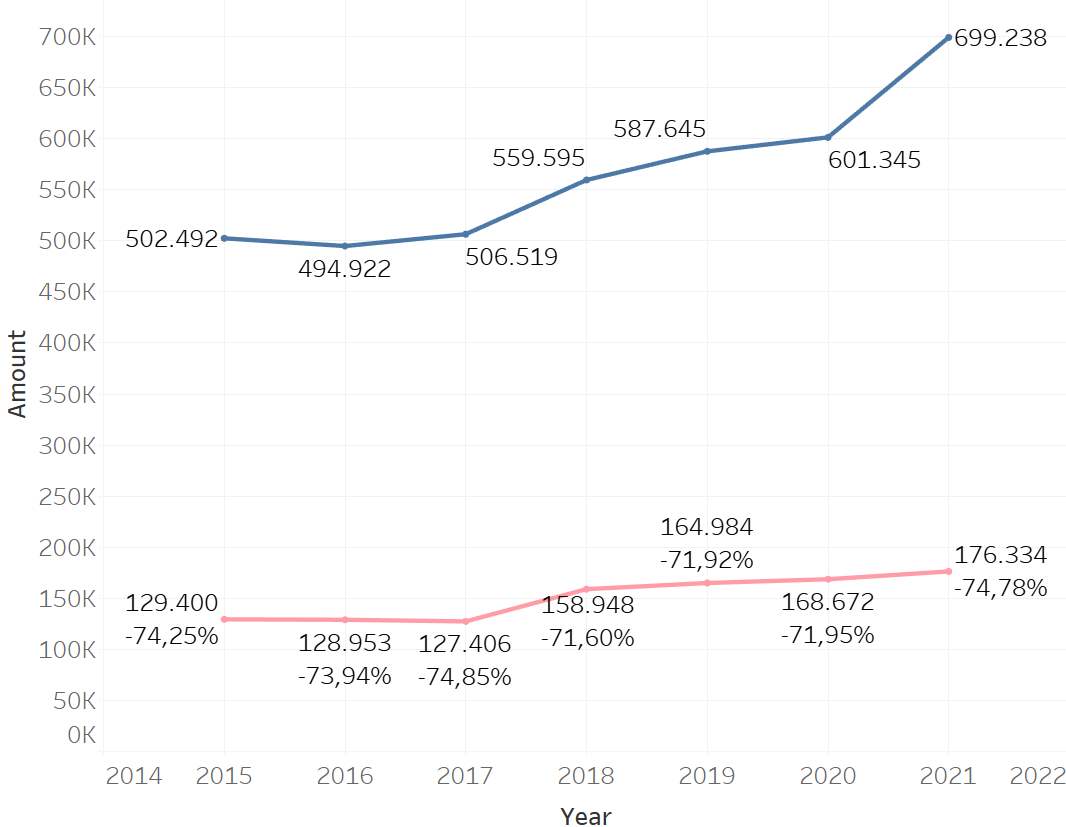
\includegraphics[width=85mm]{assets/1_qnt.PNG}
	}
	\caption{General Quantity}
	\label{fig_1_qnt}
\end{figure}

\subsubsection{Average salary}

In the graph of Figure \ref{fig_1_sal}, it is possible to verify that in all years the average salary of men is higher than that of women. This difference was smaller in 2015, which was 4.87\%. In 2021, this difference increased to 13.71\% and in 2021 it decreased again and was 11.56\%.

\begin{figure}[htbp]
	\centerline{
		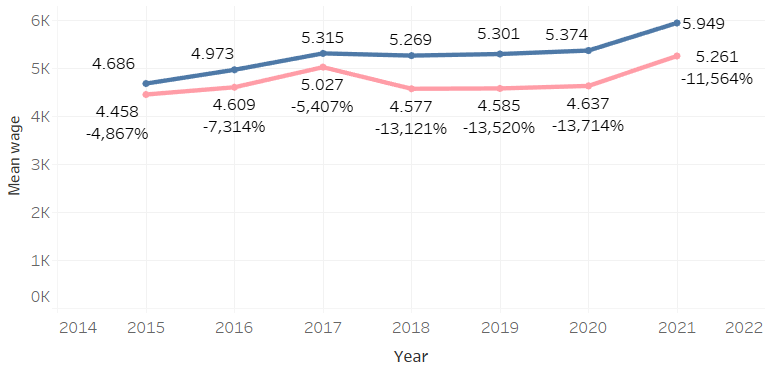
\includegraphics[width=85mm]{assets/1_sal.PNG}
	}
	\caption{Média salarial geral}
	\label{fig_1_sal}
\end{figure}


\subsection{Analysis by educational level}  \label{sub:educ}

\subsubsection{Quantity}

In Figure \ref{fig_2_qnt_educ}, it can be seen that for both genders there are more professionals with higher education compared to the number of professionals with only completed high school. The difference between the quantities of professionals by gender, both at the high school and higher education levels, varies between 71 and 78\%, being slightly higher at the high school level.

\begin{figure}[htbp]
	\centerline{
		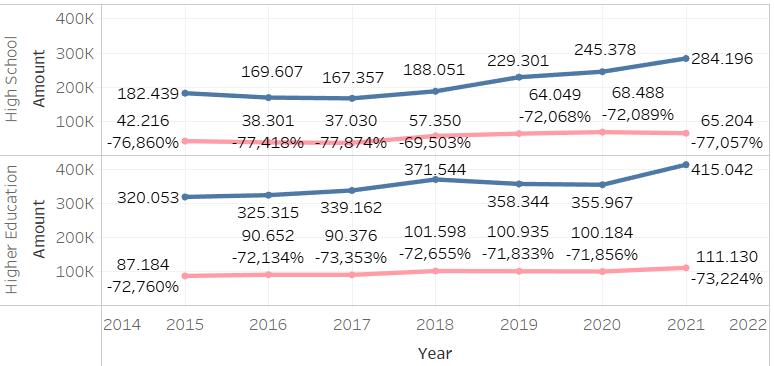
\includegraphics[width=85mm]{assets/2_qnt_educ.PNG}
	}
	\caption{Quantidade por nível educacional}
	\label{fig_2_qnt_educ}
\end{figure}

\subsubsection{Average salary}

For the average salary presented in Figure \ref{fig_2_sal_educ}, it is possible to verify that in all years the salary difference was higher at the high school level when compared to higher education. That is, women’s qualification seems to contribute to reducing wage inequality between genders in IT

\begin{figure}[htbp]
	\centerline{
		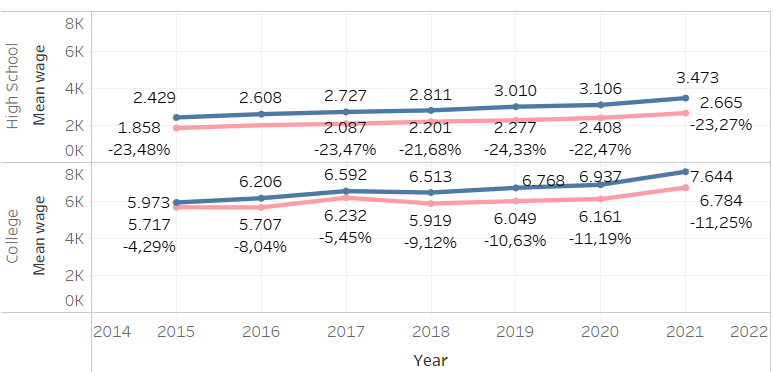
\includegraphics[width=85mm]{assets/2_sal_educ.PNG}
	}
	\caption{Média salarial por nível educacional}
	\label{fig_2_sal_educ}
\end{figure}

\subsection{Analysis by private and public sector}  \label{sub:privpub}

\subsubsection{Quantity}

In Figures \ref{fig_3_qnt_pubpriv} and \ref{fig_3_1_qnt_pubpriv}, it is possible to verify that the number of male professionals is higher than the number of female professionals, regardless of the sector. However, in the private sector the difference is even greater, as in the case of 2021, where this difference was 75.19\%, while in the public sector it was 61.09\%.

\begin{figure}[htbp]
	\centerline{
		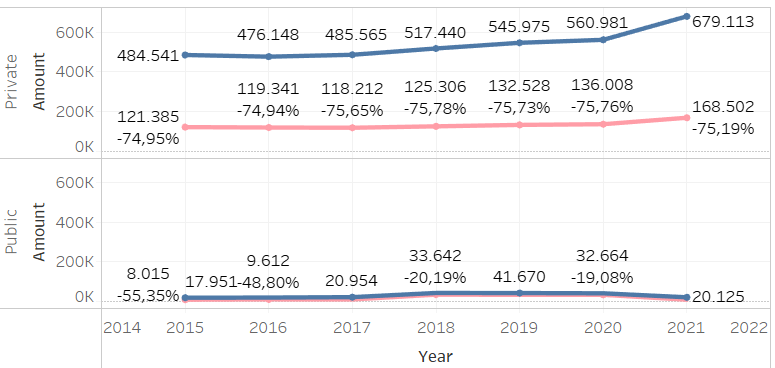
\includegraphics[width=85mm]{assets/3_qnt_pubpriv.PNG}
	}
	\caption{Quantity by sector}
	\label{fig_3_qnt_pubpriv}
\end{figure}


\begin{figure}[htbp]
	\centerline{
		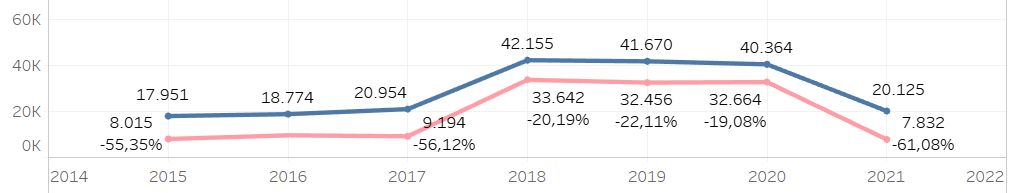
\includegraphics[width=85mm]{assets/3_1_qnt_pubpriv.PNG}
	}
	\caption{Extended quantity chart by public sector}
	\label{fig_3_1_qnt_pubpriv}
\end{figure}

\subsubsection{Average salary}

With regard to the average salaries presented in Figure \ref{fig_3_sal_pubpriv}, their percentage differences are similar when comparing the private sector with the overall picture of Figure \ref{fig_1_sal}. However, there is a much greater discrepancy in the percentage differences between 2018 and 2020 when looking at the public sector; the analyzed data does not allow for the identification of a possible cause for this phenomenon.

\begin{figure}[htbp]
	\centerline{
		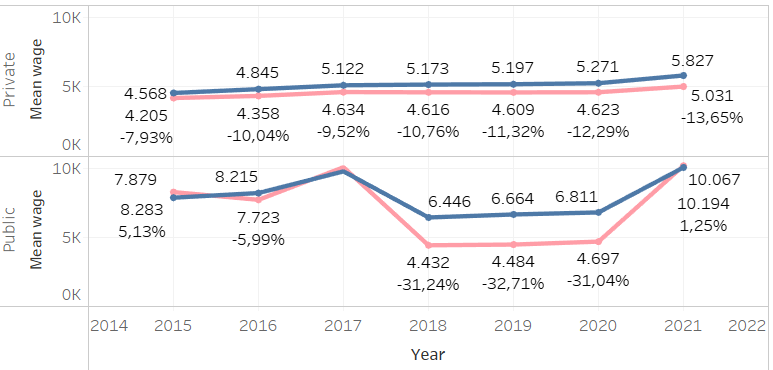
\includegraphics[width=85mm]{assets/3_sal_pubpriv.PNG}
	}
	\caption{Average salary by sector}
	\label{fig_3_sal_pubpriv}
\end{figure}

\subsection{Analysis of the amount of layoffs}

In this section, the analysis was carried out regarding the number of dismissals of male and female professionals. There is a chart for each gender. In each chart, the number of people dismissed is presented and, just below it, the number of people not dismissed, that is, kept in employment in the respective year. The percentage is also different because it analyzes the difference in relation to the previous data on its own line, not in relation to the other gender.

\subsubsection{Homem}

It is noteworthy, in Figure \ref{fig_4_qnt_h_demit}, that in 2021 the percentage of dismissal of male professionals was the highest in the last 7 years: 35.82\%. It is worth noting that 2021 was a critical year in relation to the COVID19 pandemic and that these dismissals may be related to the economic scenario of the time.

\begin{figure}[htbp]
	\centerline{
		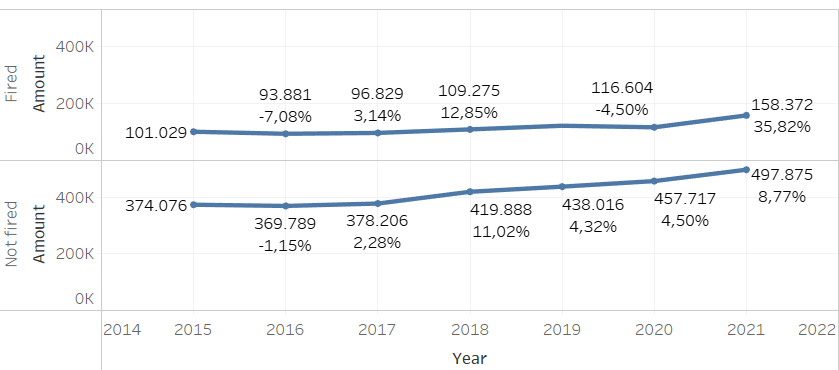
\includegraphics[width=85mm]{assets/4_qnt_h_demit.PNG}
	}
	\caption{Dismissals of men}
	\label{fig_4_qnt_h_demit}
\end{figure}

\subsubsection{Woman}

Similarly, in Figure \ref{fig_4_qnt_m_demit}, it is also possible to notice that in 2021 the percentage of dismissal of female professionals was the highest in the last 7 years: 29.91\%. This percentage is lower than that of men. Therefore, this is the only data where the asymmetry is favorable to women.

\begin{figure}[htbp]
	\centerline{
		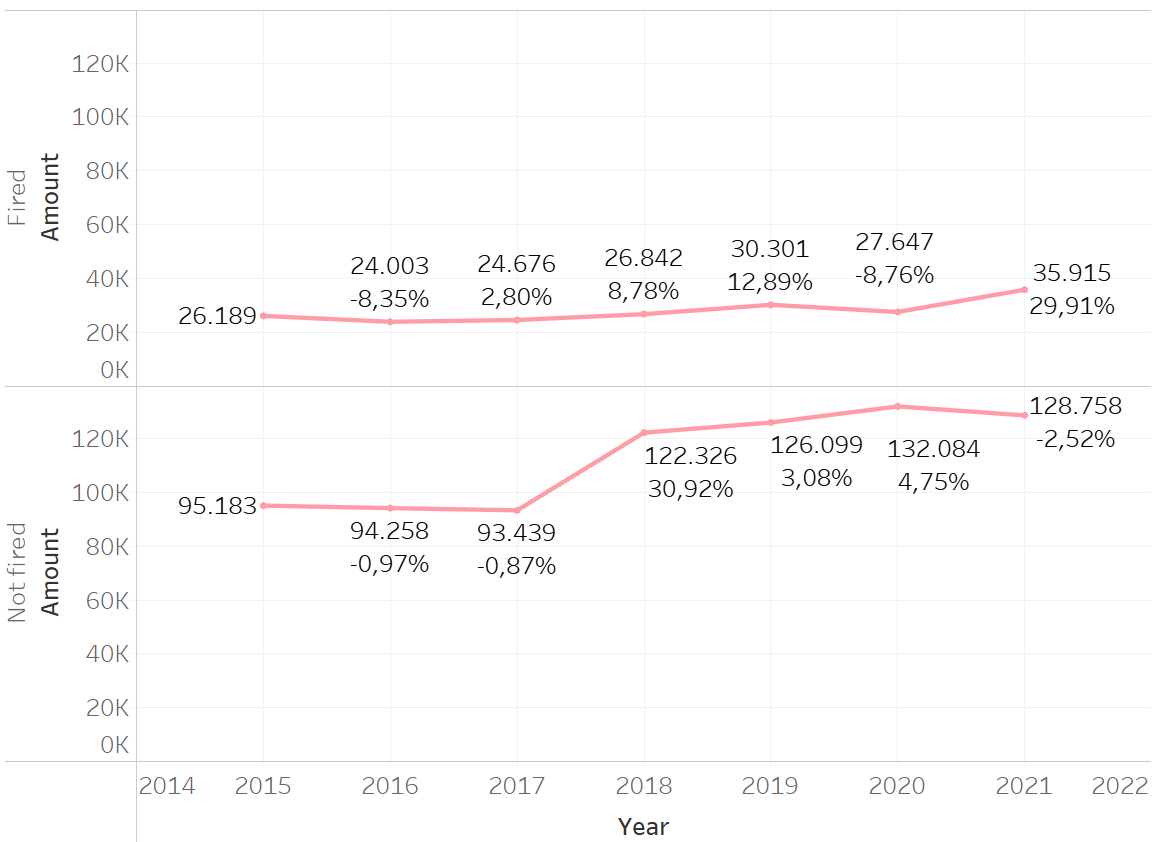
\includegraphics[width=85mm]{assets/4_qnt_m_demit.PNG}
	}
	\caption{Dismissals of women}
	\label{fig_4_qnt_m_demit}
\end{figure}

\subsection{Analysis by IT Job Title}

In the analyzes by positions, only the year 2021 was considered, as it is the last year available in our database and represents the most current data on the distribution of men and women among the various IT positions, both in the public and private sectors.

\subsubsection{Quantity}

According to Figure \ref{fig_5_qnt_cbo}, the position of Systems Development Analysts is the one that concentrates the largest number of IT professionals, both men and women, followed by Computer Support Analysts. In all professions, the number of men is greater than that of women, and the difference is greater in the position of Systems Development Analysts, where the number of men is almost 4 times greater than that of women.

\subsubsection{Average salary}

In Figure \ref{fig_5_sal_cbo}, it is possible to identify that the salary difference remains favorable for men, except for the position of Network and Data Communication Analyst, where the average salary of women is higher than that of men by 2.17\%. The largest salary difference in favor of men is related to the position of Computer Operator: 25.73\%, followed by Information Security Administrator: 19.75\% and Computer Engineer: 18.75\%. The lowest percentage differences are related to the positions of Information Systems Developer: 4.16\%, followed by Systems Development Analyst: 8.82\% and Internet Developer: 10\%. It can be concluded that the salary difference tends to be slightly lower in development areas in general.

\begin{figure}[htbp]
	\centerline{
		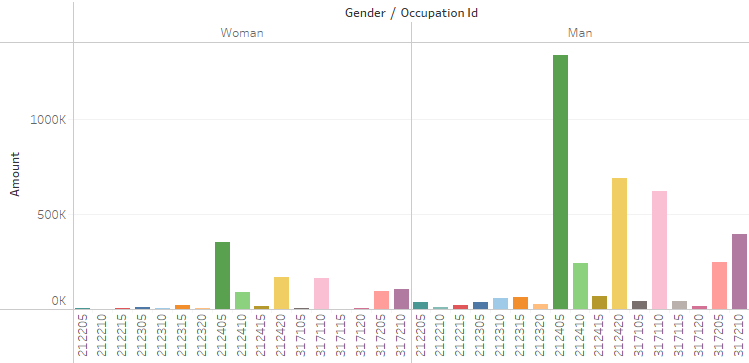
\includegraphics[width=85mm]{assets/5_qnt_cbo.PNG}
	}
	\caption{Quantity by Job in 2021}
	\label{fig_5_qnt_cbo}
\end{figure}

\begin{figure}[htbp]
	\centerline{
		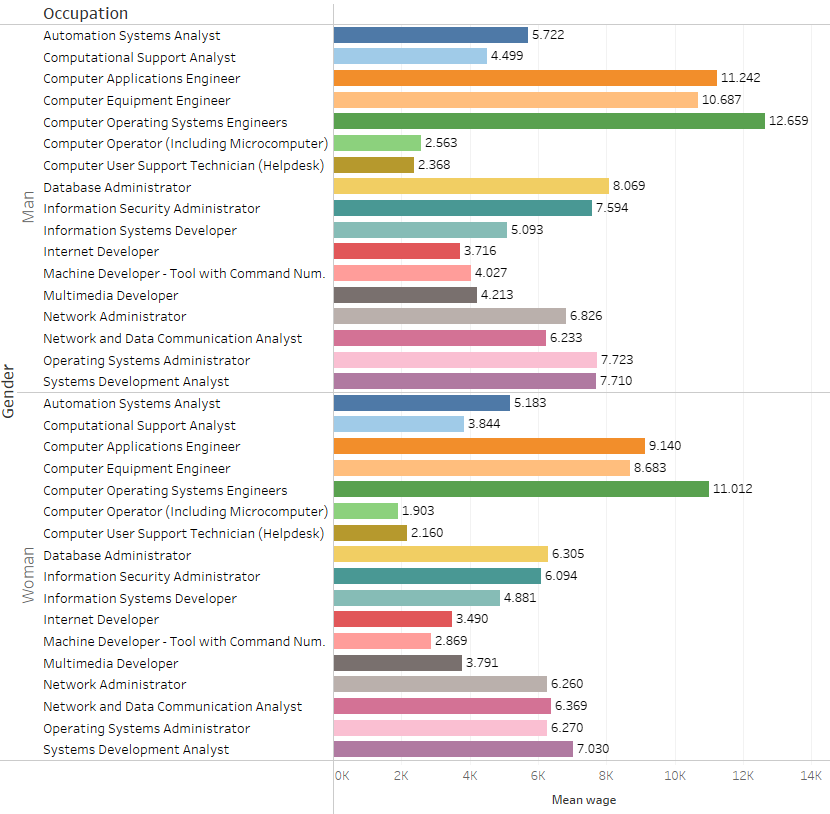
\includegraphics[width=85mm]{assets/5_sal_cbo.PNG}
	}
	\caption{Average salary per position in 2021}
	\label{fig_5_sal_cbo}
\end{figure}
\section{Considerações Finais}

O objetivo deste trabalho foi o de estudar a existência de diferenças salariais e diferenças na quantidade de demissões por gênero no setor de TI no Brasil.

Observando a população feminina e a população masculina a partir dos dados que a RAIS nos fornece, foi possível perceber que a desigualdade salarial entre gêneros evidenciadas tanto na pesquisa de 2022 do IBGE quanto na pesquisa de 2015 da ONU, aqui já citadas,  são também percebidas entre os profissionais da área de Tecnologia da Informação (TI) em todo o território brasileiro em desfavor da mulher e independentes do nível escolar, do cargo de TI e do setor onde trabalham, se público ou privado. E essa é uma realidade em todos os anos de estudo, de 2015 a 2021.

Os dados também nos permitiu evidenciar que esta é uma profissão predominantemente masculina, com uma diferença superior a 70\% em todos os anos analisados. Já com relação à quantidade de demissões, não foi possível perceber uma diferença significativa entre os gêneros, execeto em 2021, quando a porcentagem de demissões dos homens foi de 35,82\% e das mulheres doi de 29,91\%.

Os dados estudados não nos permitem esclarecer as causas dessas diferenças, apenas nos ajudam a evidenciá-las. É, portanto, necessário aprofundar os estudos no sentido de identificar os fundamentos dessas disparidades para que possam ser apontadas possíveis providências socioeconômicas e socioeducativas no sentido de mudar essa realidade. 

Dos resultados obtidos, percebe-se que há escopo para políticas específicas de crescimento da participação feminina na carreira de TI, que é considerada uma das carreiras mais promissoras da atualidade. Maiores estudos devem sugerir também o quanto da atual segregação no setor de tecnologia é gerada pelo tratamento desigual e quanto é gerada pelas preferências individuais.




 

\bibliographystyle{IEEEtran}
\bibliography{bibliografia}{}

\end{document}
